% =====================================================================
%  Assignment 1 -- Assessing climate risk at the national level: NIGER
%  Policy memo: "Why limiting climate change matters for Niger"
%  Compile with pdflatex (twice) -- works as-is on Overleaf.
% =====================================================================
\documentclass[10pt,a4paper]{article}

% ---------------------------------------------------------------------
%  1. CLIMATE IMPACT EXPLORER VALUES -- EDIT THIS BLOCK ONLY
%  Replace each \todo{...} by the number read in the CIE (Niger,
%  median across models). Example:  \newcommand{\HeatLow}{4.2}
%  Ranges are the shaded bands on the CIE chart, e.g. {2.1--6.0}.
% ---------------------------------------------------------------------
\newcommand{\AuthorName}{\todo{Your name}}
\newcommand{\CIEAccessDate}{\todo{date accessed}}

% Indicator 1 -- Land area annually exposed to heatwaves (% of land area)
\newcommand{\HeatLow}{\todo{??}}        % median at 1.5 C
\newcommand{\HeatLowRange}{\todo{??--??}}
\newcommand{\HeatHigh}{\todo{??}}       % median at 3 C
\newcommand{\HeatHighRange}{\todo{??--??}}

% Indicator 2 -- Land area annually exposed to crop failures (% of land area)
\newcommand{\CropLow}{\todo{??}}
\newcommand{\CropLowRange}{\todo{??--??}}
\newcommand{\CropHigh}{\todo{??}}
\newcommand{\CropHighRange}{\todo{??--??}}

% Indicator 3 -- Population annually exposed to river floods (% of population)
\newcommand{\FloodLow}{\todo{??}}
\newcommand{\FloodLowRange}{\todo{??--??}}
\newcommand{\FloodHigh}{\todo{??}}
\newcommand{\FloodHighRange}{\todo{??--??}}

% Figure: save your CIE screenshot as  cie_figure.png  next to this file.
% Look at the shaded uncertainty bands on that chart:
%   if the bottom of the 3 C band is ABOVE the top of the 1.5 C band
%   (the bands do not overlap), keep \bandsseparatetrue;
%   if they overlap, change it to \bandsseparatefalse.
\newif\ifbandsseparate
\bandsseparatetrue

% Set to \finaltrue once every value is filled in: removes the yellow
% highlighting (any value still missing will then show as "??").
\newif\iffinal
\finalfalse
% ---------------------------------------------------------------------

\usepackage[T1]{fontenc}
\usepackage[utf8]{inputenc}
\usepackage{tgheros}
\renewcommand{\familydefault}{\sfdefault}
\usepackage[english]{babel}
\usepackage[a4paper,top=1.5cm,bottom=1.6cm,left=1.8cm,right=1.8cm,
            headsep=0.4cm,footskip=0.7cm]{geometry}
\usepackage{microtype}
\usepackage{amssymb}
\usepackage[table]{xcolor}
\usepackage{graphicx}
\usepackage{tabularx,array,booktabs}
\usepackage{enumitem}
\usepackage{titlesec}
\usepackage{fancyhdr}
\usepackage[most]{tcolorbox}
\usepackage[hidelinks]{hyperref}
\usepackage{xurl}
\usepackage{caption}
\urlstyle{same}
\captionsetup{skip=3pt}

% ---- colours
\definecolor{navy}{HTML}{1F3A5F}
\definecolor{brick}{HTML}{A6261D}
\definecolor{lowbg}{HTML}{E8F1E8}
\definecolor{highbg}{HTML}{FBE9E6}
\definecolor{msgbg}{HTML}{F7F3EC}
\definecolor{rule}{HTML}{C9D3DF}
\definecolor{lowtxt}{HTML}{2E6B34}

% ---- placeholder macro
\iffinal
  \newcommand{\todo}[1]{??}
\else
  \newcommand{\todo}[1]{\begingroup\setlength{\fboxsep}{1pt}%
    \colorbox{yellow}{\textbf{\strut#1}}\endgroup}
\fi

% ---- typography
\setlength{\parindent}{0pt}
\setlength{\parskip}{3pt}
\linespread{1.02}
\setlist{nosep,leftmargin=1.1em,itemsep=1.5pt}
\setlist[itemize]{label={\color{navy}\small$\blacktriangleright$}}

\titleformat{\section}{\color{navy}\bfseries\large}{}{0pt}{}[{\color{rule}\titlerule[0.8pt]}]
\titlespacing*{\section}{0pt}{6pt}{2pt}

\pagestyle{fancy}
\fancyhf{}
\renewcommand{\headrulewidth}{0pt}
\fancyhead[L]{\scriptsize\color{gray}Policy memo \,|\, Niger \,|\, UNFCCC negotiating team}
\fancyhead[R]{\scriptsize\color{gray}\AuthorName}
\fancyfoot[R]{\scriptsize\color{gray}\thepage}

\newcommand{\degC}{\,\textdegree C}
\newcommand{\low}{1.5\degC}
\newcommand{\high}{3\degC}
\newcolumntype{Y}{>{\raggedright\arraybackslash}X}
\newcolumntype{C}[1]{>{\centering\arraybackslash}p{#1}}
\newcolumntype{L}[1]{>{\raggedright\arraybackslash}p{#1}}

\begin{document}

% =====================================================================
%  HEADER
% =====================================================================
\begin{tcolorbox}[colback=navy,colframe=navy,arc=0pt,boxrule=0pt,
                  left=8pt,right=8pt,top=6pt,bottom=7pt]
{\color{white!70!navy}\scriptsize\bfseries POLICY MEMO \textbullet{} FOR OFFICIAL USE}\\[2pt]
{\color{white}\LARGE\bfseries Why limiting climate change matters for Niger}
\end{tcolorbox}
\vspace{-4pt}
{\small
\begin{tabularx}{\linewidth}{@{}l Y l Y@{}}
\textbf{To:}   & Minister of Environment, Head of Niger's UNFCCC delegation &
\textbf{From:} & \AuthorName, Climate Adviser \\
\textbf{Date:} & 14 October 2026 &
\textbf{Re:}   & What Niger stands to lose, and to gain if warming is limited \\
\end{tabularx}}

% =====================================================================
%  a) KEY MESSAGE
% =====================================================================
\vspace{2pt}
\begin{tcolorbox}[colback=msgbg,colframe=brick,boxrule=0pt,leftrule=3pt,arc=0pt,
                  left=7pt,right=7pt,top=4pt,bottom=4pt]
{\color{brick}\small\bfseries KEY MESSAGE}\\[1pt]
\textbf{Niger's economy rests on the activities that heat and erratic rain hit first: rain-fed farming
and herding generate almost 40\% of GDP and employ more than 80\% of the population.}
Climate Impact Explorer projections show that at \high{} of global warming rather than \low,
the share of Niger's land hit by a heatwave in a typical year would rise from about \HeatLow\% to
\HeatHigh\%, and the share exposed to crop failure from \CropLow\% to \CropHigh\%. The World Bank
estimates that a dry, high-impact climate future could cut Niger's GDP by up to 11.9\% by 2050.
\textbf{Niger emits a negligible share of global greenhouse gases yet faces some of the largest
losses: pushing for a rapid global phase-out of emissions is a matter of national interest, not charity.}
\end{tcolorbox}

% =====================================================================
%  WHY NIGER IS EXPOSED
% =====================================================================
\section{Why Niger is unusually exposed}
\begin{itemize}
  \item \textbf{An open-air economy.} Agriculture and livestock account for almost 40\% of GDP and
        over 80\% of jobs, and depend overwhelmingly on rainfall (World Bank, 2024).
  \item \textbf{Shocks are already frequent and costly.} The 2005 and 2010 droughts triggered national
        food crises; the 2024 floods killed 339 people and affected more than 1.1~million (AFP, 2024).
  \item \textbf{Demand is growing fast.} With one of the fastest-growing populations in the world,
        Niger needs more food, water and jobs every year, from a climate that makes each harder to secure.
\end{itemize}

% =====================================================================
%  b) THREE PRIORITY IMPACTS
% =====================================================================
\section{Three priority impacts: \low{} versus \high{} of global warming}
{\footnotesize\itshape Source: Climate Impact Explorer (Climate Analytics), Niger, multi-model median;
model range in brackets. A \high{} world is roughly where current policies lead by 2100; the
difference between the two columns is what Niger gains if the world limits warming.\par}
\vspace{3pt}

{\small
\renewcommand{\arraystretch}{1.25}
\begin{tabularx}{\linewidth}{@{}L{3.25cm} C{2.05cm} C{2.05cm} Y@{}}
\rowcolor{navy}
\color{white}\bfseries Impact (CIE indicator) &
\color{white}\bfseries At \low &
\color{white}\bfseries At \high &
\color{white}\bfseries Why it matters for Niger \\[2pt]
%
\textbf{1. Extreme heat}\newline{\footnotesize\itshape Land area exposed to heatwaves each year (\%)} &
\cellcolor{lowbg}\textbf{\HeatLow\%}\newline{\footnotesize [\HeatLowRange]} &
\cellcolor{highbg}\textbf{\HeatHigh\%}\newline{\footnotesize [\HeatHighRange]} &
Farming, herding and construction are done outdoors, mostly without electricity or cooling. Heat cuts
working hours, stresses livestock and raises mortality: GIZ/PIK (2021) project about 50 more very
hot days a year and a threefold rise in heat-related deaths by 2080 under high emissions. \\
\midrule
\textbf{2. Crop failure}\newline{\footnotesize\itshape Land area exposed to crop failure each year (\%)} &
\cellcolor{lowbg}\textbf{\CropLow\%}\newline{\footnotesize [\CropLowRange]} &
\cellcolor{highbg}\textbf{\CropHigh\%}\newline{\footnotesize [\CropHighRange]} &
Millet and sorghum feed the country. Past warming has already cut West African millet yields by
10--20\% (Sultan et al., 2019), and beyond about +2\degC{} of local warming no plausible increase in
rainfall offsets the heat losses (Sultan et al., 2013). A failed harvest means higher grain prices,
malnutrition and distress sales of livestock. \\
\midrule
\textbf{3. River floods}\newline{\footnotesize\itshape Population exposed to river floods each year (\%)} &
\cellcolor{lowbg}\textbf{\FloodLow\%}\newline{\footnotesize [\FloodLowRange]} &
\cellcolor{highbg}\textbf{\FloodHigh\%}\newline{\footnotesize [\FloodHighRange]} &
Niamey, the Niger River valley and irrigated rice schemes concentrate people, infrastructure and
food production. In 2020 the river reached its highest level since 1929 and paralysed the capital
(Al Jazeera, 2020). Niger must prepare for droughts \emph{and} floods, often in the same decade. \\
\bottomrule
\end{tabularx}}
\vspace{2pt}

% =====================================================================
%  c) VISUAL
% =====================================================================
\begin{figure}[t]
\centering
\IfFileExists{cie_figure.png}{%
  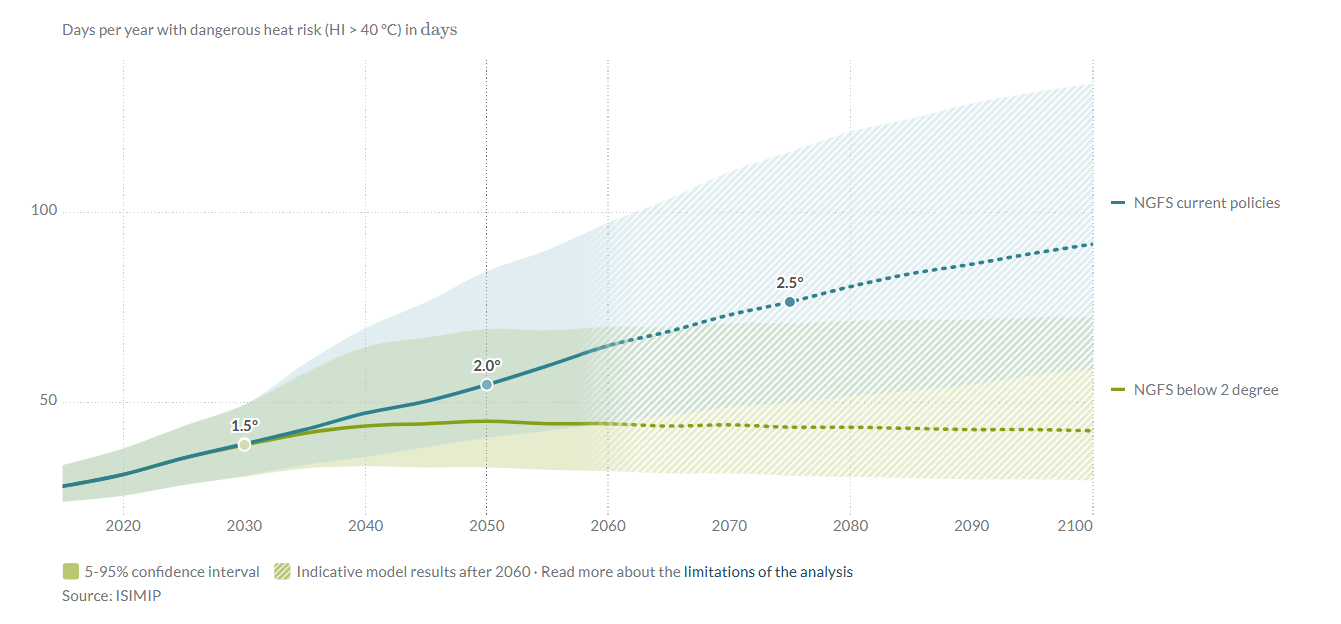
\includegraphics[width=0.86\linewidth,height=6.6cm,keepaspectratio]{cie_figure.png}%
}{%
  \fcolorbox{gray}{gray!8}{\parbox[c][5.6cm][c]{0.84\linewidth}{\centering\small
  \todo{Save your Climate Impact Explorer screenshot as \textsf{cie\_figure.png}}\\[4pt]
  Niger -- land area exposed to crop failure -- \low{} vs.\ \high{} (or 1.5\degC{} pathway
  vs.\ current policies)}}%
}
\vspace{-2pt}
\caption*{\footnotesize\textbf{Figure 1. Crop-failure exposure in Niger: the gap between the two curves is
what limiting warming saves.} At \high, about \CropHigh\% of Niger's land would be exposed to crop failure
in a typical year, against \CropLow\% at \low.
\ifbandsseparate
  The shaded bands show model uncertainty: even the low end of the \high{} range lies above the
  high end of the \low{} range, so the direction of the risk is robust.
\else
  The shaded bands show model uncertainty and overlap: the exact size of the increase is uncertain,
  but the central estimate is clearly worse at \high.
\fi
Source: Climate Impact Explorer, Climate Analytics.}
\end{figure}
\vspace{-10pt}

% =====================================================================
%  d) NATIONAL INTEREST
% =====================================================================
\section{Implications for Niger's national interest}

\textbf{1. The cost is counted in GDP points.} The World Bank (2022) estimates that by 2050 climate
change would reduce Niger's annual GDP by 2.2\% in a wet, optimistic scenario but by 11.9\% in a dry,
pessimistic one, the largest loss among the five G5 Sahel countries. These figures are probably
\emph{under}estimates: they leave out migration, conflict and ecosystem degradation.

\textbf{2. The real danger is a cascade, not a single number.} A hot year with erratic rains
$\rightarrow$ failed harvests and pastures $\rightarrow$ higher grain prices and forced sales of
livestock $\rightarrow$ malnutrition, household debt, migration to cities and farmer--herder tensions
$\rightarrow$ emergency spending that crowds out investment. The warmer the world, the more often these
``bad years'' occur.

\textbf{3. Adaptation has limits that only global mitigation can push back.} Irrigation, drought-tolerant
seeds and crop insurance are essential but costly, and beyond roughly +2\degC{} of local warming they cannot
fully offset heat losses (Sultan et al., 2013). Every tenth of a degree avoided lowers an adaptation
bill Niger cannot pay alone.

\begin{tcolorbox}[colback=lowbg,colframe=lowtxt,boxrule=0pt,leftrule=3pt,arc=0pt,
                  left=7pt,right=7pt,top=3pt,bottom=3pt]
\textbf{Recommended negotiating position.}
(i)~Defend the 1.5\degC{} goal and press major emitters for NDCs consistent with a rapid fossil-fuel
phase-out; (ii)~tie Niger's support to scaled-up, accessible adaptation finance with simplified access
for Least Developed Countries; (iii)~use the Loss and Damage Fund for droughts and floods, in coalition
with the African Group and the LDC group.
\end{tcolorbox}

\section{What the evidence does, and does not, say}
{\small
Rising heat is the most robust signal: all models agree on its direction. \textbf{For rainfall, models
disagree even on the sign of change}, and some project small millet yield gains from CO$_2$ fertilisation
(GIZ/PIK, 2021). The risk to plan for is therefore not a certain fall in average yields but greater
variability, with more drought years \emph{and} more flood years. These figures are projections, not
forecasts, and they describe hazards only: Niger's high social vulnerability means actual impacts are
likely to be larger than the physical numbers suggest.\par}

% =====================================================================
%  REFERENCES (page 3 -- outside the 2-page limit)
% =====================================================================
\clearpage
\section{References}
{\small
\begin{list}{}{\leftmargin=1.2em \itemindent=-1.2em \itemsep=4pt \parsep=0pt}
\item AFP (2024, 9 October). Niger ups flood toll to 339 dead, more than 1 million affected.
      \emph{Inquirer.net}. \url{https://globalnation.inquirer.net/251812/niger-ups-flood-toll-to-339-dead-more-than-1-million-affected}
\item Al Jazeera (2020, 29 August). Niger flooding: At least 45 killed, 226,000 displaced.
      \url{https://www.aljazeera.com/news/2020/08/niger-flooding-45-killed-226000-displaced-200829064145712.html}
\item Climate Analytics (2026). \emph{Climate Impact Explorer}: Niger. Indicators: land area exposed to
      heatwaves, land area exposed to crop failures, population exposed to river floods.
      \url{https://climate-impact-explorer.climateanalytics.org} (accessed \CIEAccessDate).
\item GIZ \& PIK (2021). \emph{Climate Risk Profile: Niger}. Bonn and Potsdam: Deutsche Gesellschaft für
      Internationale Zusammenarbeit and Potsdam Institute for Climate Impact Research.
      \url{https://www.adaptationcommunity.net/wp-content/uploads/2021/02/GIZ_Climate-risk-profile-Niger_EN_final.pdf}
\item Sultan, B., Defrance, D., \& Iizumi, T. (2019). Evidence of crop production losses in West Africa due
      to historical global warming in two crop models. \emph{Scientific Reports}, 9, 12834.
\item Sultan, B., Roudier, P., Quirion, P., Alhassane, A., Muller, B., Dingkuhn, M., Ciais, P., Guimberteau, M.,
      Traore, S., \& Baron, C. (2013). Assessing climate change impacts on sorghum and millet yields in the
      Sudanian and Sahelian savannas of West Africa. \emph{Environmental Research Letters}, 8, 014040.
\item World Bank (2022). \emph{G5 Sahel Region Country Climate and Development Report}. CCDR Series.
      Washington, DC: World Bank. \url{http://hdl.handle.net/10986/37620}
\item World Bank (2024, 28 June). The World Bank supports food security and climate resilience for households
      in Niger [Press release].
      \url{https://www.worldbank.org/en/news/press-release/2024/07/01/the-world-bank-supports-food-security-and-climate-resilience-for-households-in-niger}
\end{list}}

\end{document}
